\begin{pastexam}[label={px:nccu-108-dsa-07}]{政大資科所 108 學年度 第 7 題}
（問答）

(10\%) Give a balanced binary search tree containing the following data: 1, 2, 3, 4, 5, 6, 7.
\end{pastexam}

\begin{pastsoln}
$7 = 2^3 - 1$ 個數，可以排成一棵完美平衡（滿的）二元搜尋樹，高度 $2$：根取中位數 $4$，左子樹由
$1, 2, 3$ 遞迴（根 $2$），右子樹由 $5, 6, 7$ 遞迴（根 $6$）。
\begin{center}
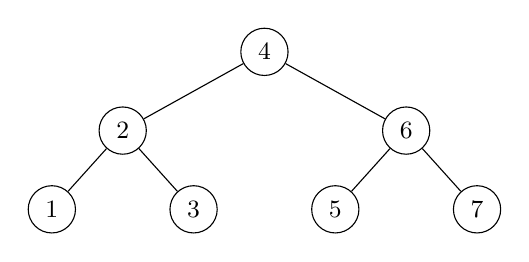
\begin{tikzpicture}[x=1cm,y=1cm,v/.style={circle,draw,minimum size=6mm,inner sep=0pt,font=\small}]
\node[v] (4) at (0,0) {4};
\node[v] (2) at (-1.8,-1) {2}; \node[v] (6) at (1.8,-1) {6};
\node[v] (1) at (-2.7,-2) {1}; \node[v] (3) at (-0.9,-2) {3};
\node[v] (5) at (0.9,-2) {5}; \node[v] (7) at (2.7,-2) {7};
\draw (4)--(2) (4)--(6) (2)--(1) (2)--(3) (6)--(5) (6)--(7);
\end{tikzpicture}
\end{center}

\textbf{檢查}。 二元搜尋樹性質：$4$ 的左子樹 $\{1, 2, 3\}$ 都比 $4$ 小、右子樹 $\{5, 6, 7\}$ 都比 $4$ 大；
$2$ 的左右是 $1 < 2 < 3$，$6$ 的左右是 $5 < 6 < 7$。 中序走訪得 $1, 2, 3, 4, 5, 6, 7$，由小到大（資結書
定理~9.1）。 平衡：每個節點左右子樹的高度都相同（差 $0$），所以它同時是 AVL 樹（資結書第~10.2~節），
也可以把所有節點塗黑當成紅黑樹（每條到 \NIL 的路徑都有 $3$ 個黑節點）。 高度 $2 = \lfloor \lg 7
\rfloor$，是 $7$ 個節點的二元樹能有的最小高度，搜尋任何一個數最多比 $3$ 次。

\textbf{怎麼建}。 數已經排好時，取中間的當根、左右兩半遞迴，$O(n)$ 就能建出高度 $\lfloor \lg n \rfloor$
的樹。 如果是依序把 $1, 2, \ldots, 7$ 插入一般的二元搜尋樹，會得到一條往右的鏈（高度 $6$），不平衡；
插入 AVL 樹則經過幾次左旋，最後恰好也是上面這棵樹。
\end{pastsoln}
